\section{Slow Controls}

The CLAS12 slow controls system was heavily upgraded for the 12 GeV era at JLab.  It incorporates legacy and modern hardware and standalone controls systems into full EPICS integration, such that everything is accessible from a single interface and on any computer in the CLAS12 system.  Another important aspect is leveraging standard infrastructure tools supported by central JLab computing resources, for a manageable and reliable controls system.

The CLAS12 slow controls system is based on Experimental Physics Industrial Control System (EPICS), currently version 3.14.12.5 \cite{epics-website}, and includes about 90 EPICS input-output controllers (IOCs) interfacing with approximately 50 different types of hardware via various communication protocols and 100K(?) process variables (PVs).

The controls system monitors and controls all aspects of the CLAS12 detector, beamline, and magnet systems, with monitoring on the DAQ system.  This includes power supplies from a variety of manufacturers, programmable logic controllers, cryogenic and gas systems, multiple scaler hardwares, flasher sytems, all of the VXS crates, trigger system performance, beamline motors, with sequencing for more complex operations like polarimetry and magnet hystereses.  An example of the superconducting torus magnet's nitrogen system and 10~kHz EPICS monitoring is shown in Fig.\ref{fig:tordaq}, and one of the scaler displays covering multiple CLAS12 detector systems is shown in Fig.\ref{fig:jlabscalers}.

\begin{figure}[htbp]\centering
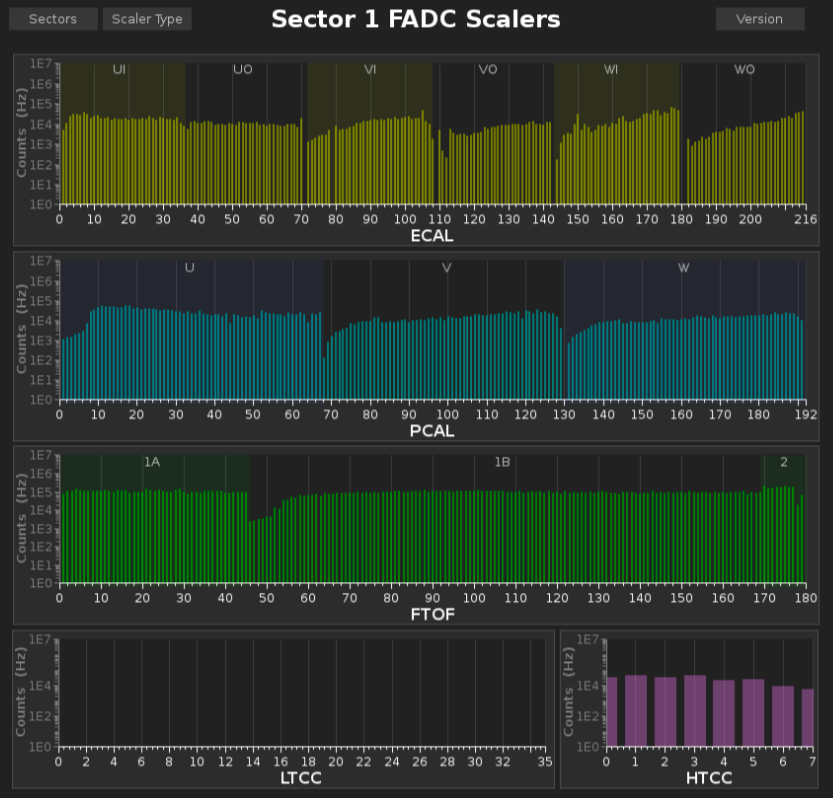
\includegraphics[width=8cm]{img/fd-scalers}
\caption{And example of the JLab FADC250 scalers for CLAS12 PMT-based detector systems.\label{fig:jlabscalers}}
\end{figure}

\begin{figure*}[t]\centering
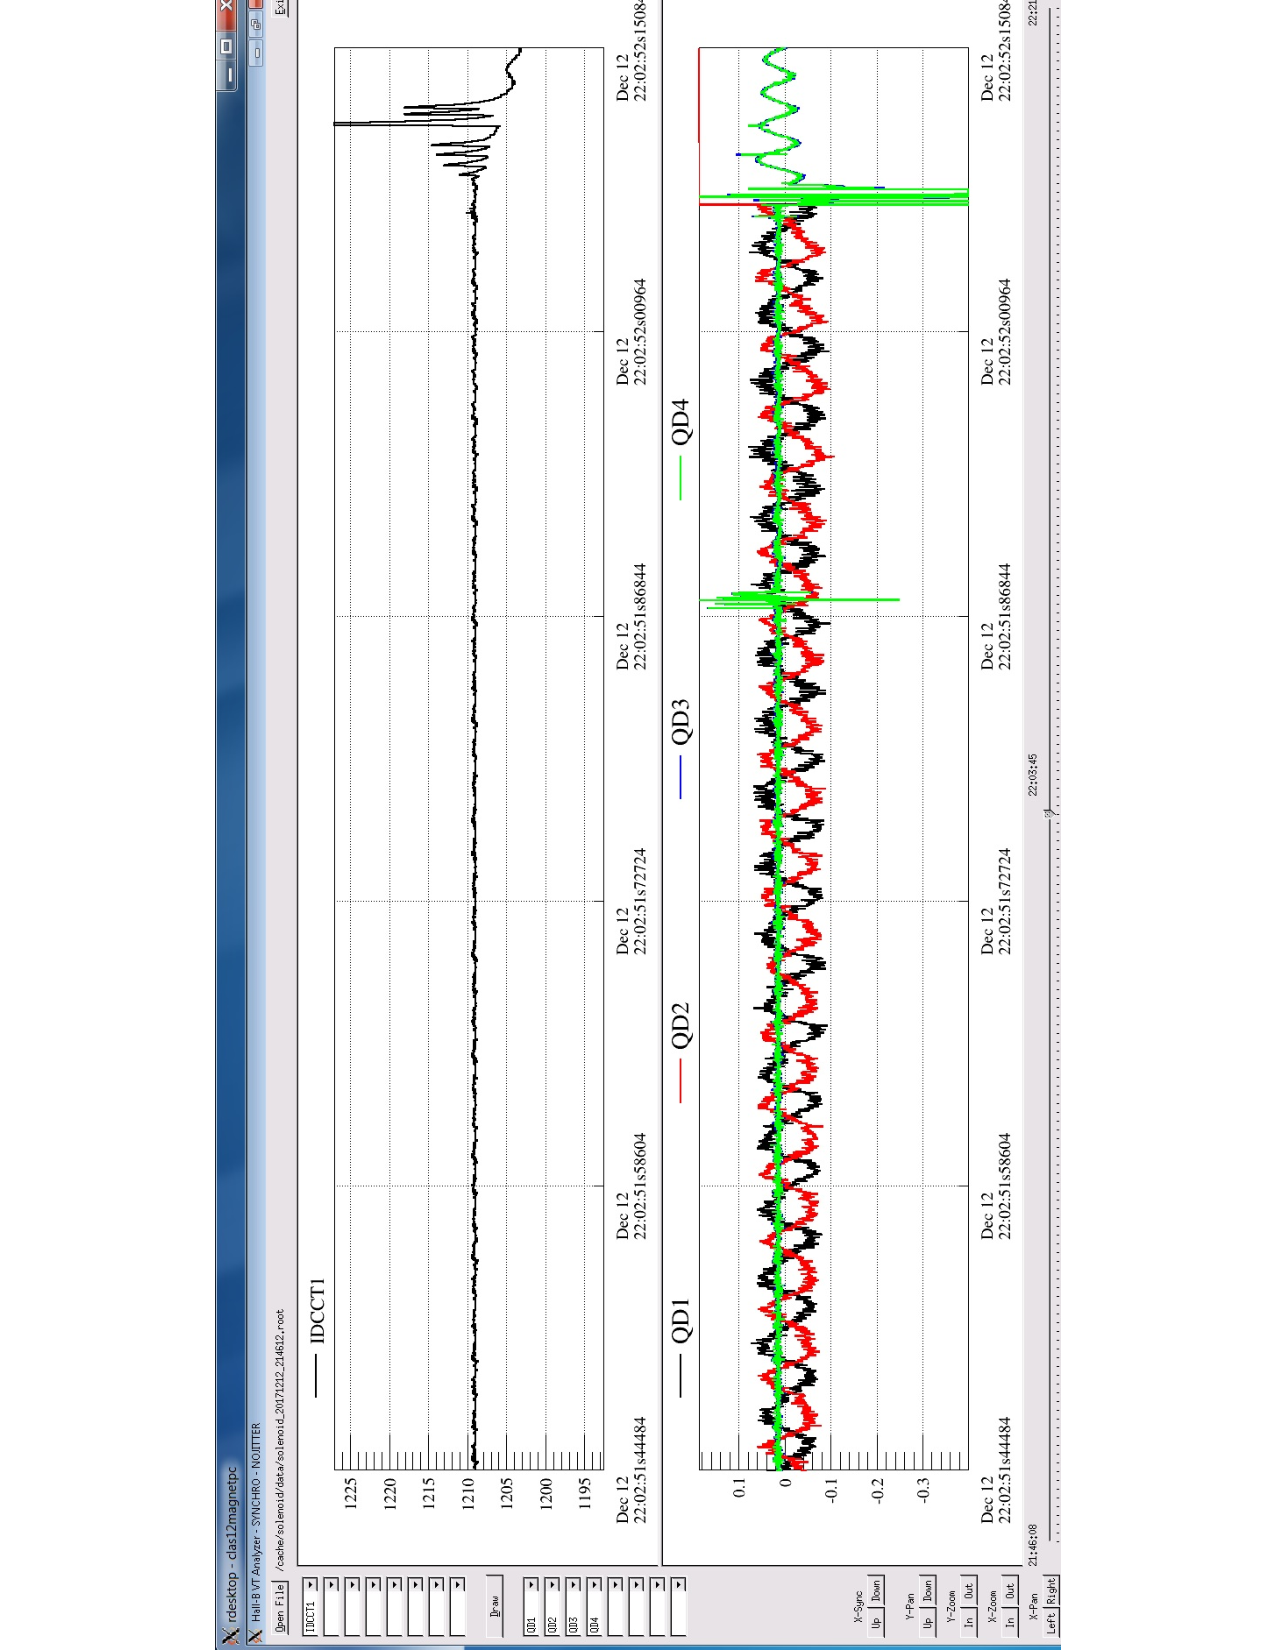
\includegraphics[width=0.9\textwidth]{img/tordaq}
\caption{The 10 kHz EPICS-based readout of superconducting magnet's quench detection system.\label{fig:tordaq}}
\end{figure*}

Most of the IOCs run on standard rack-mounted servers running Red Hat Enterprise 7 (RHEL7) in the Control Room.  A few IOCs run in more specialized systems in the experimental hall, such as VxWorks 5.X real-time operating systems on Motorolla VME controllers, primarily for high-rate, synchronous beam monitoring and support of legacy components.  All IOCs and associated processes are managed with procServ for interactive access when necessary and cronjobs for automatic startup and recovery \cite{procserv-website}.

For the graphical user interface we chose the modern Control Systems Studio (CS-Studio) developed at Oak Ridge National Laboratory \cite{css-website}.   CS-Studio is an Eclipse-based suite of tools for developing and monitoring large-scale control systems.  It includes various features supporting quick interface development, such as templating and dynamic generation.

We also use the CS-Studio alarm system.  It is based on a MYSQL database for storing alarm configurations, status, and message history, combined with a server monitoring the IOCs, updating the database, and communicating with clients.  The clients include a graphical interface tightly integrated with the rest of the controls system, with visible feedback and heirarchical view of the alarm system, an annuciator service running in the background in the Control Room, and a notifier service sending emails to on-call experts on particular alarm conditions.

The operators of the controls system run directly on desktop PCs running RHEL7.  Full remote access is also provided, via 2-factor authentication and X-forwarding or VNC, as well as VMWare virtual machines supported by JLab.  Read-only access in a web browser is provided via WebOPI, another product affiliated with CS-Studio.

We utilize two internal EPICS channel access gateways, one read-only for the web interface, and the other for minimizing connections to superconducting magnet controls systems.  Wherever appropriate, the standard autosave feature of EPICS is utilized to automatically preserve settings across IOC reboots, and the standard Burt save/restore mechanisms.  The controls system also utilizes many custom hardware and software interlocks.

An important component of the slow controls system is archiving data.  For this we utilize the EPICS archiving system called Mya, a product developed by and in support of accelerator operations at JLab and shared with the experimental halls.  This provides storage and access to many previous years data of all CLAS12 EPICS PVs \cite{mya}.

Installation and configuration of the associated desktop and server machines, including custom service daemons, cron jobs, IOCs, network disk mounting, and deployment of upgrades and software changes, is managed via puppet and a central server maintained by JLab \cite{puppet-website}. The resulting maintainence is almost hands-free, and recovery from hardware failures or power outages is largely automated.  Monitoring of the servers is performed with Nagios, also provided by JLab, which provides email notifications about system errors \cite{nagios-website}.

